\documentclass[14pt]{extarticle}
\usepackage{amsmath}
\usepackage{amssymb}
\usepackage{graphicx}
\usepackage{tikz}
\usetikzlibrary{trees}
\usepackage{graphicx}
\graphicspath{ {../chap03/} }
\usepackage[top=0.75in, bottom=0.75in, left=0.75in, right=0.75in]{geometry}
\newcommand*{\Scale}[2][4]{\scalebox{#1}{\ensuremath{#2}}}%
\usepackage[shortlabels]{enumitem}
% \usepackage{showframe}


\begin{document}
	
\section*{Announcements}
Students who do not meet prerequisites according to PAWS will be automatically dropped from the course as of Wednesday, January 27th. If you are not sure if you meet the course prerequisites, contact one of the
undergraduate advisors.

\section*{Math 208 Sections 3.1 and 3.2}

\subsection{Homework and other}
\begin{itemize}
\item Sections 3.1, 3.2
\item Sections 4.1, 4.2
\end{itemize}

\subsection{Goals}

\begin{itemize}
	\item Review Syllabus
	\item Gain fluency using Canvas
	\item Find unknown values using the formulas for 
	\begin{enumerate}[(i)]
		\item Simple interest,
		\item Compound interest, and
		\item Continuous compound interest.
	\end{enumerate}
	\item Recall logarithm rules
	\item State and apply formula for Annual Percentage Yield
\end{itemize}

\subsection{Syllabus}

\subsection{Canvas}
\begin{itemize}
	\item Video introduction
	\item Quiz 1
\end{itemize}

\subsection{Breakout}
Download or view the Icebreaker instructions from Canvas.

\subsection{Section 3.1: Simple Interest}
Interest is the cost of using money. When you borrow money, you pay interest. When you lend money, you earn interest. Simple interest is the foundation for other interest types. In real life it is mostly used for terms of up to one year. At the end of the term, The interest is paid along with the principal.
\begin{align*}
	I = &Prt \tag{1} \\
	&A = P+I= P+ Prt \\
	A = &P + Prt \tag{2} \\
	A = &P(1+rt) \tag{3} \\
	&I = \text{ Interest} \\
	&A = \text{ Amount / Future value} \\
	&P = \text{ Principal / Present value} \\
	&r = \text{ decimal annual interest rate} \\
	&t = \text{ time in years}	
\end{align*}
\textbf{NOTE:} Interest rates are always converted to decimal form before use in formulas.
\subsubsection*{Examples}
\begin{itemize}
	\item \textbf{Problem 50}: If \$5000 is loaned for a term of 9 months at a 6.2\% annual rate, how much interest is earned?
	\begin{align*}
		I= &Prt \\
		&P = 5000 \\
		&r = 0.065 \\
		&t = 9/12 = 0.75 \\
		I =& \$5000 \times 0.065 \times 0.75 \\
		= &  \$232.50
	\end{align*}
	\item \textbf{Problem 40}: Given $A = \$410, P = \$400, r=10\%$, find $t$.
	\begin{align*}
		A &= P(1+rt) \\
		A/P &= 1+ rt \\
		rt & = A/P - 1 \\
		t &= \frac{A/P - 1}{r} \\
		&= \frac{410/400 - 1}{0.10} \\
		&= \frac{0.025}{0.10} \\
		t &= 0.25 \text{ yrs} = 3 \text{ months}
	\end{align*}
\end{itemize}

\subsection{Section 3.2}
Say that at the end of a term, the principal along with the interest is reinvested. This underlies the concept of compounding interest. Such that at the end of each compounding period, interest is added to the principal and the rate of return is now applied to that compounded total.
\subsubsection*{Compound Interest}
\begin{align*}
	A = &P(1+i)^n \tag{4} \\
	A = &P\left(1+\frac{r}{m}\right)^{mt} \tag{5} \\
	&A = \text{ Amount / Future value} \\
	&P = \text{ Principal / Present value} \\
	&i = \text{ decimal rate per compounding period} \\
	&n = \text{ total number of compounding periods} \\
	&r = \text{ decimal annual nominal interest rate} \\
	&m = \text{ number of compounding periods per year} \\
	&t = \text{ time in years} \\
	&\text{Note that } i=r/m \text{ and } n= mt
\end{align*}
\textbf{Examples}
You should be able to solve for any unknown value given the other values.
\begin{itemize}
	\item \textbf{Problem 10}: Using equation (4), find the future value of $P=\$2800, i=0.003$, and $n=24$?
	\begin{align*}
		A = &P(1+i)^n \\
		&= 2800(1+0.003)^{24} \\
		&= 2800 \times 1.07454 \\
		A &= \$3008.71 \\
	\end{align*}
	\item \textbf{Problem 38C}: If \$2000 is invested at 7\% compounded monthly, what is the amount after 5 years? How much interest is earned?
	\begin{align*}
		A = &P\left(1+\frac{r}{m}\right)^{mt} \\
		&P =2000 \\
		&r = 0.07 \\
		&m = 12 \text{ compounding periods in a year} \\
		&t = 5 \text{ years} \\
		A = &2000(1+0.07/12)^{12 \times 5} 	= 2000(1.005833)^{60} \\
		A = &\$2835.19 \\\\
		I = &A-P \\
		I = &2835.19 - 2000 = \$835.19
	\end{align*}
\end{itemize}

\subsubsection*{Continuous Compound Interest}
Consider when the compounding period gets smaller and smaller, i.e. minutes then seconds. As the compounding period get smaller, m gets larger. Taking the limit of this we have continuous compounding. We will look at this more in Chapter 9.
\begin{align*}
	A = &Pe^{rt} \tag{6} \\
	&A = \text{ Amount / Future value} \\
	&P = \text{ Principal / Present value} \\
	&e = \text{ irrational constant known as Euler's number} \\
	&r = \text{ decimal annual nominal interest rate} \\
	&t = \text{ time in years}
\end{align*}
\textbf{Examples}
You should be able to solve for any unknown value given the other values.
\begin{itemize}
	\item \textbf{Problem 16}: Using equation (6), find the present value of $A=\$19000, r=7.69\%$, and $t=5$ years?
	\begin{align*}
		A &= Pe^{rt} \\
		P &= \frac{A}{e^{rt}} \\
		&= \frac{19000}{e^{0.0769 \times 5}} = \frac{19000}{e^{0.3845}} = \frac{19000}{1.4689} \\
		P &= \$12935.03
	\end{align*}
\end{itemize}

\subsection{Logarithm Rules}
These are from algebra but you will need these to solve a variety of problems. In our notation, log is logarithm base 10 and ln is logarithm base e (natural log).
\begin{align*}
&\text{Product } &	&log(A * B) = log(A) + log(B) \\
&\text{Quotient } &	&log(A / B) = log(A) - log(B) \\
&\text{Power } &	&log(A^p) = p * log(A) \\
&\text{Indentity } &	&log(10) = 1 \\
&\text{Indentity } &	&ln(e) = 1 \\
&\text{Zero } &	&log(1) = 0
\end{align*}
\textbf{Examples}
You will need these to solve for the exponent, $t$.
\begin{itemize}
	\item \textbf{Problem 57}: How long will it \$6000 to grow to \$8600 if it is invested at 9.6\% compounded continuously?
	\begin{align*}
		A &= Pe^{rt} \\
		A/P &= e^{rt} \\
		\ln(A/P) &= \ln(e^{rt}) = rt \ln(e) \\
		rt &= \ln(A/P) \\
		t &= \frac{\ln(A/P)}{r} \\
		t &= \frac{\ln(8600/6000)}{0.096} = \frac{\ln(1.433)}{0.096} = \frac{0.36}{0.096} \\
		t &\approx 3.75 \text{ years}
	\end{align*}
	\item \textbf{Problem 62A}: How long will it take money to double if it is invested at $8\%$ compounded semiannually?
	\begin{align*}
		A = &P\left(1+\frac{r}{m}\right)^{mt} \\
		A/P &= \left(1+\frac{r}{m}\right)^{mt} \\
		&A/P =2 \\
		&r = 0.08 \\
		&m = 2 \text{ compounding periods in a year} \\
		\log(A/P) &= \log\left(\left(1+\frac{r}{m}\right)^{mt}\right) \\
		&= mt \log\left(1+\frac{r}{m}\right) \\
		mt &= \frac{\log(A/P)}{\log\left(1+\frac{r}{m}\right)} \\
		t &= \frac{\log(A/P)}{m\log\left(1+\frac{r}{m}\right)} \\
		&= \frac{\log(2)}{2\log\left(1+\frac{0.08}{2}\right)} = \frac{0.30103}{2\log(1.04)} = \frac{0.30103}{2(0.01703)} \\
		t &\approx 8.836 \text{ years}
	\end{align*}
\end{itemize}

\cleardoublepage

\subsection{Annual Percentage Yield}
In order to easily compare different rates and compounding periods, it is useful to convert them to similar terms. This is the \textit{Annual Percentage Yield (APY)}, which is the simple interest rate that produces the same return in one years term.
\begin{align*}
	APY &= (1+r/m)^m -1 &\text{for compounding}\tag{7} \\
	APY &= e^r -1 &\text{for continuous compounding}\tag{8}
\end{align*}
\textbf{Examples}
\begin{itemize}
	\item \textbf{Problem 54}: What is the APY for money invested at an annual rate of A) 3.05\% compounded quarterly and B) 2.95\% compounded continuously? Which investment is better?
	\begin{align*}
		APY_{quaterly} &= (1+r/m)^m -1 \\
		&= (1+0.0305/4)^4 -1 = 1.007625^4 -1\\
		&= 3.085\% \\\\
		APY_{continuous} &= e^r -1 \\
		&= e^0.0295 -1 \\
		& =2.994\% \\
	\end{align*}
	The better investment is that which compounds quarterly.
\end{itemize}

\cleardoublepage
\subsection{Summary and Comparison}
Below is a graph that shows a comparison between 
\begin{itemize}
	\item Simple interest $(r=7\%)$, the green line
	\item Compound interest $(r= 4\%, m = 2)$, the red line
	\item Continuous compound interest $(r=4\%)$, the black line
\end{itemize} 
Over time, the compound interest always beats simple interest, in this example after about 26 years. The difference between the compound interest and the continuous compound interest is not so clear and depends on $m$. The best way to compare these is to use APY.
\\\\
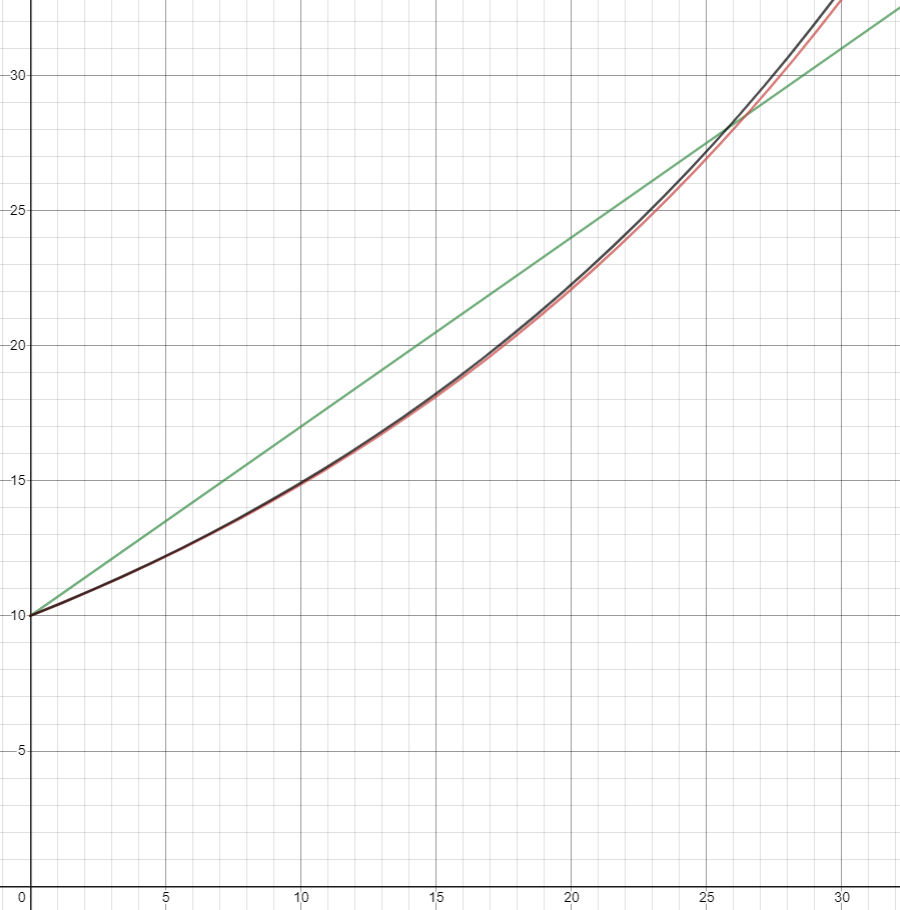
\includegraphics[width=0.85\linewidth]{3-1}

\end{document}
